\section{Cost: A Model and What the Runs Say About It}
\label{sec:cost}

The book keeps three terms apart: \textbf{cost} is what it takes to own and operate hardware, \textbf{price} is what a provider charges for a service, and \textbf{quality} is how good the generated textbook is. This section concerns cost and the price a generation service would have to charge. It is a model with stated assumptions, and its purpose here is narrower than a business case: to check whether its inputs and its predicted run times survive contact with measured runs.

\subsection{The Model}

The model adds up what one unit costs to buy, set up, and run per year, divides by the hours it spends generating, and multiplies by the machine time a book needs. Table~\ref{tab:costassume} lists the assumptions. Three are the author's: the three benchmark stages are 10\% of the cost of a whole book, the service keeps a 20\% margin on price, and a unit generates half of its hours. The rest were chosen by the assistant and are labeled assumed.

\begin{table}[htbp]
\centering
\small
\begin{tabular}{@{}p{4.3cm}p{4.3cm}p{6.6cm}@{}}
\toprule
\textbf{Item} & \textbf{Value} & \textbf{Basis} \\
\midrule
Hardware plus accessories & \$7,200 & List price of a 128~GB unit in October 2026, plus a power supply and cabling; 3-year life, no resale \\
Setup labor & 40 h at \$90 & Assumed \\
Operations labor & 4 h per month at \$90 & Assumed: updates, new models, restarting failed runs \\
Electricity & 150 W generating, 40 W idle, \$0.1385/kWh & Assumed; not measured at the wall on these units \\
Network and space & \$20 per month & Assumed \\
Generating share of hours & 50\% & Author's assumption \\
Three-stage workload & 200,000 output tokens, 280 turns, 15 s overhead per turn & Assumed, from one measured stage and the published book's size \\
Three stages as a share of a book & 10\% & Author's assumption; untested \\
Margin & 20\% of price & Author's assumption \\
\bottomrule
\end{tabular}
\caption{Cost-model assumptions.}
\label{tab:costassume}
\end{table}

Under these assumptions one unit costs \$8,275 a year to own and run, of which people are two thirds and electricity about one percent, and each generating hour costs \$1.89. The reference case is a 30.7-billion-parameter dense model at 34 tokens per second: a whole book takes 28 machine hours, costs \$53, and would have to sell for \$66 to leave a 20\% margin. Two features of the model are worth stating plainly. Nearly all of the cost is fixed, so the cost of a book is close to the yearly cost divided by the number of books produced; and a faster model saves less than its speed suggests, because for the fastest models the per-turn overhead is longer than the generation time.

\subsection{Measured Time Against Predicted Time}

The model predicts the machine time for the three stages as 200,000 tokens divided by decode speed plus 280 turns times the per-turn overhead. At the time it was written only one stage had been measured. The runs now allow the comparison in Table~\ref{tab:costcompare}.

\begin{table}[htbp]
\centering
\small
\begin{tabular}{@{}lrrrrr@{}}
\toprule
\textbf{Model} & \textbf{Predicted (h)} & \textbf{Measured (h)} & \textbf{Ratio} & \textbf{Cost} & \textbf{Per 1K words} \\
\midrule
\Gtwentysix & 1.7 & 1.8 & 1.07 & \$3.44 & \$0.13 \\
\Qsix & 1.7 & 2.2 & 1.29 & \$4.16 & \$0.06 \\
\Nemo & 1.7 & 2.7 & 1.57 & \$5.04 & \$0.06 \\
\Gptoss & 2.5 & 1.9 & 0.76 & \$3.62 & \$0.20 \\
\Gthirtyone & 2.8 & 4.8 & 1.71 & \$9.07 & \$0.34 \\
\Qeight & 9.1 & 5.6 & 0.61 & \$10.54 & --- \\
\bottomrule
\end{tabular}
\caption{Predicted and measured machine time for the three stages. Predictions are the model's, in which \Qsix{} and \Nemo{} take the speed of \Gtwentysix{} by assumption, and \Qeight{} is predicted at its measured per-turn overhead of 90 s. Cost is measured time at the model's \$1.89 per generating hour and so inherits its 50\% duty-cycle assumption. Per 1K words divides that cost by thousands of words in written chapters; \Qeight{} wrote none.}
\label{tab:costcompare}
\end{table}

The predictions were within a factor of 1.7 of the measurement in all six cases, and the errors have no single direction. That is a plausibility check and not a validation, because the books differ in size, from 10 to 14 chapters and from 18,000 to 82,000 written words, whereas the model assumed a 13-chapter, 55,000-word book, and because its inputs were each off in both directions. The assumed 200,000 output tokens compare with 108,000 to 532,000 measured across the three stages, and the assumed 280 turns with 93 to 678. The two models that completed every chapter produced 437,000 and 532,000 tokens, more than twice the assumption, and wrote books 40\% to 50\% longer than the reference. Rerunning the model's formula with the measured tokens and turns, at the model's decode speeds, over-predicts the three fast sparse models by 1.4 to 1.6 times (2.6, 3.2, and 4.2 hours against 1.8, 2.2, and 2.7). The reason is the per-turn overhead, the least stable input. Back-solved from the measurements it is 7 to 9 seconds for those three models against the 15 assumed, 22 seconds for \Gptoss, about 40 seconds for \Gthirtyone{} (inflated by one stopped run), and about 100 seconds for \Qeight, close to the 90 seconds the model took from its one measured stage. The close agreement in Table~\ref{tab:costcompare} is therefore partly the offsetting of errors.

The model's rule for assumed speeds is also testable. It predicted 34 tokens per second for \Qeight{} by analogy with \Gthirtyone; the measurement was 26. It reported that miss when it was found, which is why the other assumed speeds, six of the ten, can be taken at face value only as assumptions.

\paragraph{Implied cost of a whole book.}
If the three stages are 10\% of a book, as the model assumes, the measured times imply whole-book costs of about \$34 for \Gtwentysix, \$36 for \Gptoss, \$42 for \Qsix, \$50 for \Nemo, and \$91 for \Gthirtyone, and the price at a 20\% margin is a quarter higher. The 10\% share has not been tested: no local model has attempted MicroSims, the glossary, the FAQ, or quizzes here. If a model cannot build working MicroSims, the other 90\% of a book has no price at all.

\subsection{Sensitivity}

Figure~\ref{fig:cost} varies one assumption at a time. Demand and labor move the answer far more than hardware does. A unit that generates a quarter of the time costs twice as much per book as one that generates half, and a unit that generates a tenth of the time costs five times as much; cutting the hardware price from \$6,950 to \$3,999 moves the cost by about \$6. The share assumed for the three stages is the largest single uncertainty, because it scales every other number.

\begin{figure}[htbp]
\centering
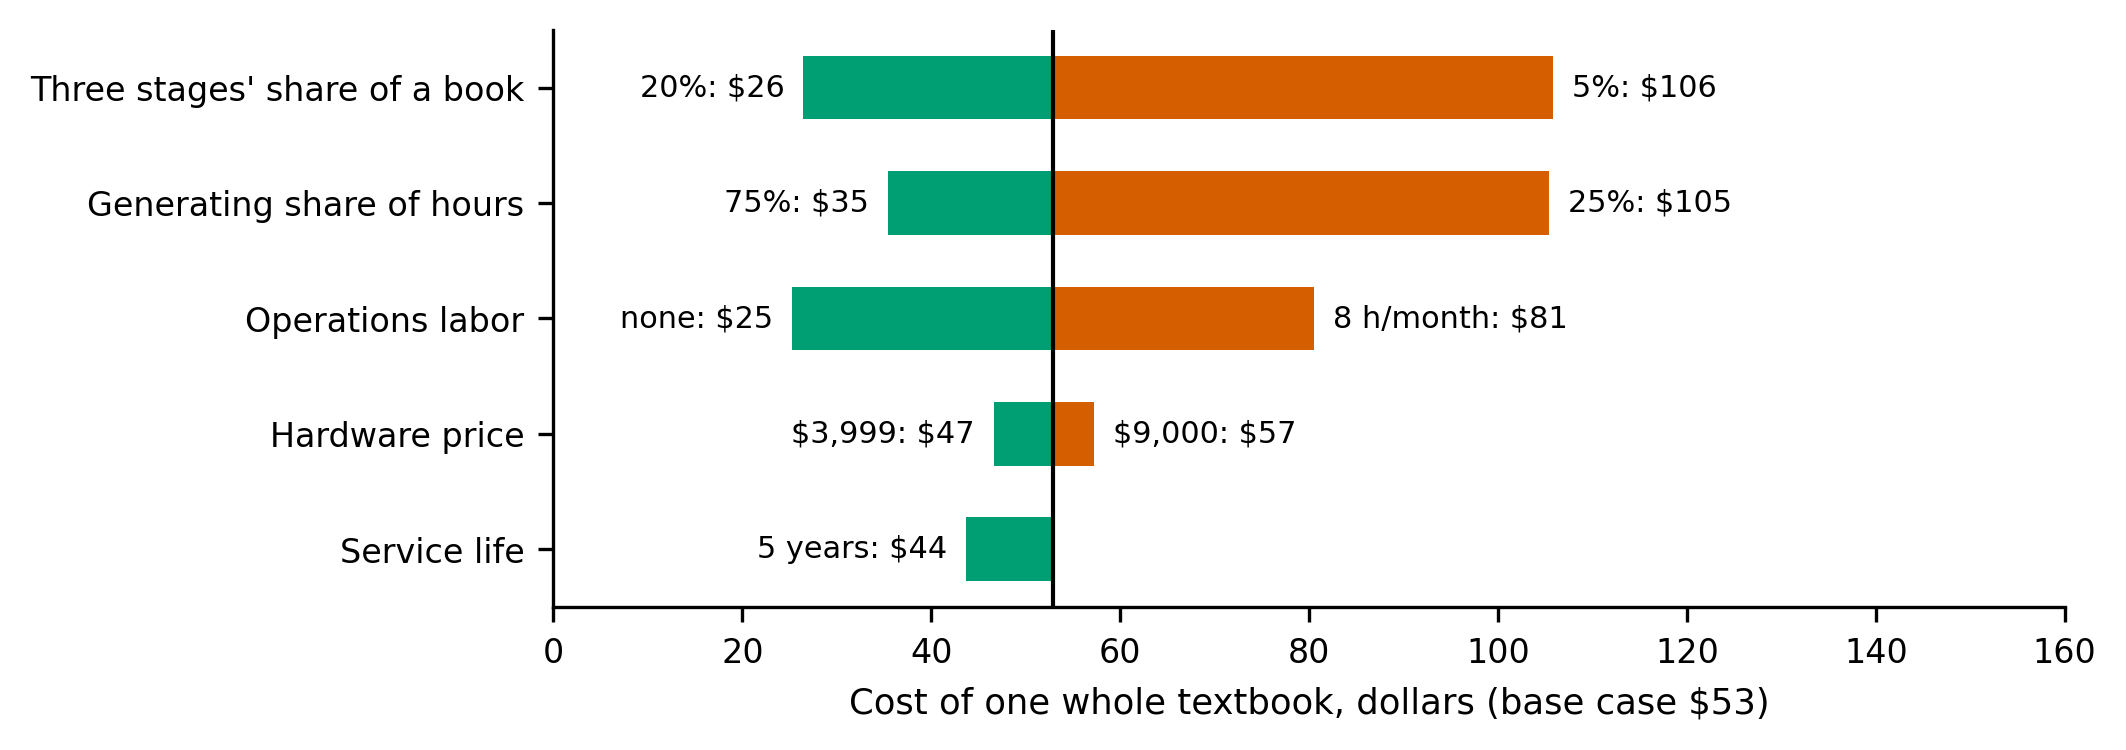
\includegraphics[width=0.95\textwidth]{figures/fig-cost-sensitivity.png}
\caption{One-at-a-time sensitivity of the cost of a whole textbook to each assumption, around the reference case. Bars to the left reduce the cost; bars to the right increase it.}
\label{fig:cost}
\end{figure}

\subsection{What the Price Leaves Out}

The model prices generation only. It excludes human review: ten hours of review by a subject expert at \$90 an hour adds \$900, seventeen times the cost of generating the book, and no output has yet been reviewed. It excludes the cloud supervision that started and watched these runs, which a service would replace with scripts at a cost not counted; it excludes selling, financing, and tax; and it excludes license terms, since several candidates state no license or attach conditions to commercial use. It also excludes a comparison with cloud generation of the same book, which would need token counts and timings that were not recorded for the published reference.
